\documentclass[a4paper,12pt]{article}

\usepackage[utf8]{inputenc}
\usepackage[left=0.5in,right=0.5in,top=1in,bottom=1in]{geometry}
\usepackage{amsmath,amssymb,amsfonts}
\usepackage{pgfplots,graphicx,calc,changepage}
\pgfplotsset{compat=newest}
\usepackage{enumitem}
\usepackage{fancyhdr}
\usepackage[colorlinks = true, linkcolor = blue]{hyperref}

% Syntax highlighting
\usepackage{listings}
\usepackage{xcolor}

\definecolor{codegreen}{rgb}{0.40,0.62,0.07}
\definecolor{codegray}{rgb}{0.5,0.5,0.5}
\definecolor{codeblue}{rgb}{0.09,0.57,0.73}
\definecolor{backcolour}{rgb}{1,1,1}

\lstdefinestyle{mystyle}{
    backgroundcolor=\color{backcolour},   
    commentstyle=\color{codegreen},
    keywordstyle=\color{magenta},
    numberstyle=\tiny\color{codegray},
    stringstyle=\color{codeblue},
    basicstyle=\ttfamily\small,
    breaklines=true,                     
    keepspaces=true,                 
    numbers=left,                    
    numbersep=5pt,                  
    showspaces=false,
    showstringspaces=false,
    showtabs=false,                  
    tabsize=4
}

\lstset{style=mystyle}

\newcommand{\nats}{\mathbb{N}}
\newcommand{\reals}{\mathbb{R}}
\newcommand{\rats}{\mathbb{Q}}
\newcommand{\ints}{\mathbb{Z}}
\newcommand{\comps}{\mathbb{C}}
\newcommand{\pols}{\mathcal{P}}
\newcommand{\cants}{\Delta\!\!\!\!\Delta}
\newcommand{\eps}{\varepsilon}
\newcommand{\st}{\backepsilon}
\newcommand{\abs}[1]{\left| #1 \right|}
\newcommand{\dom}[1]{\mathrm{dom}\left(#1\right)}
\newcommand{\for}{\text{ for }}
\newcommand{\dd}{\mathrm{d}}
\newcommand{\spn}{\mathrm{sp}}
\newcommand{\nul}{\mathcal{N}}
\newcommand{\col}{\mathrm{col}}
\newcommand{\rank}{\mathrm{rank}}
\newcommand{\norm}[1]{\lVert #1 \rVert}
\newcommand{\inner}[1]{\left\langle #1 \right\rangle}
\newcommand{\pmat}[1]{\begin{pmatrix} #1 \end{pmatrix}}
\renewcommand{\and}{\text{ and }}

\newsavebox{\qed}
\newenvironment{proof}[2][$\square$]
    {\setlength{\parskip}{0pt}\par\textit{Proof:} #2\setlength{\parskip}{0.25cm}
        \savebox{\qed}{#1}
        \begin{adjustwidth}{\widthof{Proof:}}{}
    }
    {
        \hfill\usebox{\qed}\end{adjustwidth}
    }

\pagestyle{fancy}
\fancyhead{}
\lhead{Caleb Jacobs}
\chead{APPM 5600: Numerical Analysis I}
\rhead{Homework \#12}
\cfoot{}
\setlength{\headheight}{35pt}
\setlength{\parskip}{0.25cm}
\setlength{\parindent}{0pt}

\begin{document}
\section*{Problems}
\begin{enumerate}[label = \arabic*)]
	\item 
	\begin{enumerate}[label = (\alph*)]
		\item Write a code to approximate 
		\[
			\int_{-5}^5 \frac{1}{1 + x^2} \;\dd x
		\]
		using composite trapezoidal rule and composite Simpson's rule. 
		
		\begin{center}
			\emph{Code is attached at the end of the document.}
		\end{center}
		
		\item To can compute the number of intervals to use for the trapezoidal rule to get an error less than $ 10^{-4} $ we first need to maximize the second derivative of our integrand over the interval from -5 to 5:
		\[
			M = \max_{x \in [-5,5]} \abs{\frac{\dd^2}{\dd x^2} \frac{1}{1 + x^2}} = \max_{x \in [-5,5]} \abs{\frac{2(3 x^2 - 1)}{(x^2 + 1)^3}} = 2.
		\]
		Next, we can obtain $ n $ as
		\[
			\frac{(b - a)^3 M}{12 n^2} = \frac{10^3 2}{12 n^2} < 10^{-4} \implies n > 1290.99.
		\]
		So, we will take $ n_T = 1291 $.
		
		Similarly, we can find $ n $ for Simpson's rule by, first, maximizing the fourth derivative of our integrand as
		\[
			M = \max_{x \in [-5,5]} \abs{\frac{\dd^4}{\dd x^4} \frac{1}{1 + x^2}} = \max_{x \in [-5,5]} \abs{\frac{24(5 x^4 - 10x^2 + 1)}{(x^2 + 1)^5}} = 24.
		\]
		Then, we can compute $ n $ from the error bound as
		\[
			\frac{(b - a)^5 M}{180 n^4} = \frac{10^5 24}{180 n^4} < 10^4 \implies n > 107.457.
		\]
		So, take $ n_S = 108 $.
		
		\item Running my code gives me the following results:
		\begin{table}[h!]
			\centering
			\begin{tabular}{c|ccc}
				Method & Runtime (s) & \# Func. Evals. & Result \\
				\hline \\[-2ex]
				Trapezoidal & $ 6.70 \cdot 10^{-5} $  & 1292 & 2.7468014 \\
				Simpson's    & $ 3.80 \cdot 10 ^{-5} $ & 109    & 2.7478015 \\
				Quad $ \varepsilon = 10^{-4} $ & $ 1.79 \cdot 10^{-4} $ & 41 & 2.7467951 \\
				Quad $ \varepsilon = 10^{-6} $ & $ 2.08 \cdot 10^{-4} $ & 81 & 2.7468013
			\end{tabular}
		\end{table}
	
		From the table, we can see that in every case, \lstinline[language = matlab]!quad(...)! uses less function evaluations than both composite trapezoidal and composite Simpson's. The lower number function evaluations can be attributed to \lstinline[language = matlab]!quad(...)! using an adaptive Simpson's rule which will, hopefully, optimize the nodes that we need function evaluations at to get a desired accuracy. As a result of the adaptive nodes used in \lstinline[language = matlab]!quad(...)!, we should also expect a longer runtime to find the optimal nodes instead of just using equilength intervals like trapezoidal and regular Simpson's. In fact, we do see the longer runtimes in the table. So even though \lstinline[language = matlab]!quad(...)! uses less function evaluations, it still takes longer to find the optimal nodes. 
		
		Another interesting observation comes with the accuracy of trapezoidal and Simpson's rule. Even though we computed the required number of intervals to use to obtain an error of $ 10^{-4} $ both trapezoidal and Simpon's achieved a good few more digits accuracy than the required error tolerance. This better convergence is due to the error bounds being just that, bounds on the error. In other words, the worst our error could be with our chosen number of intervals is $ 10^{-4} $ but in practice we will do a little better.
	\end{enumerate}

	\item Using my code, I was able to obtain the convergence plot below
	\begin{figure}[h!]
		\centering
		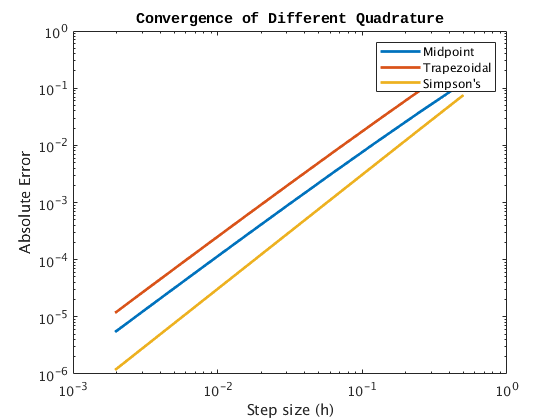
\includegraphics[width = 0.75\textwidth]{images/Convergence.png}
	\end{figure}
	
	Just as expected from our computed error bounds in class, we see that both midpoint and trapezoidal rule converge at the same rate with the error of the midpoint rule being slightly better. Furthermore, we can see that Simpson's rule has a higher convergence rate than both midpoint and trapezoidal rule which is right in line with the error bounds we found in class.
	
	\begin{center}
		\emph{Code is attached at the end of the document.}
	\end{center}
\end{enumerate}

\newpage
\section*{Code Used}
\subsection*{Problem 1}
\rule{\textwidth}{4pt}
	\lstinputlisting[language = matlab]{code/Problem1.m}
\rule{\textwidth}{4pt}

\newpage
\subsection*{Problem 2}
\rule{\textwidth}{4pt}
	\lstinputlisting[language = matlab]{code/Problem2.m}
\rule{\textwidth}{4pt}
\end{document}